\section{Coordinate Descent Reconstructions on Simulated Data}
Here we test the Coordinate Descent algorithm on two simulated datasets and show we indeed only need a subset of the Fourier Transform Matrix' columns $F^{-1}$. The datasets contain idealized MeerKAT observations. Compared to the real world, the two simulated datasets contain few Visibilities and not representative of the real data volume. Also, more realistic simulations which contain pointing-, calibration-, and thermal noise are out of scope for this project. The simulations are used to isolate the two fundamental issues in radio interferometer image reconstruction: Non-uniform sampling and incomplete measurements.

We compare the reconstruction quality to CASA's CLEAN implementation. Coordinate Descent was able to produce a super-resolved version of the simulated measurements, reconstructing point sources above the accuracy limit of MeerKAT.

\subsection{Super-resolution of two point sources}
The first simulated observation contains two non-zero pixels, i.e. point sources, with intensity of 2.5 and 1.4 Jansky/Beam, with a resolution of 0.5 arc-seconds per pixel. The resolution of the image is therefore higher than MeerKAT. An ideal compressed sensing reconstruction would create an image where all pixels are zero except for the two point sources. Figure \ref{results:points} shows the reconstructed images of CLEAN and Coordinate Descent.

CLEAN reconstructs the image \ref{results:points:tclean} at the accuracy limit of the instrument. It essentially reconstructs a blurred version of the observed image, where the blurring represents the accuracy of the instrument. With compressed sensing, we aim to reconstruct a de-blurred image. The image \ref{results:points:cd} shows the Coordinate Descent reconstruction, which creates two much narrower peaks than CLEAN. This is an example of super resolution. Coordinate Descent located structures smaller than the accuracy of MeerKAT would allow.

\begin{figure}[h]
	\centering
	\begin{subfigure}[b]{0.4\linewidth}
		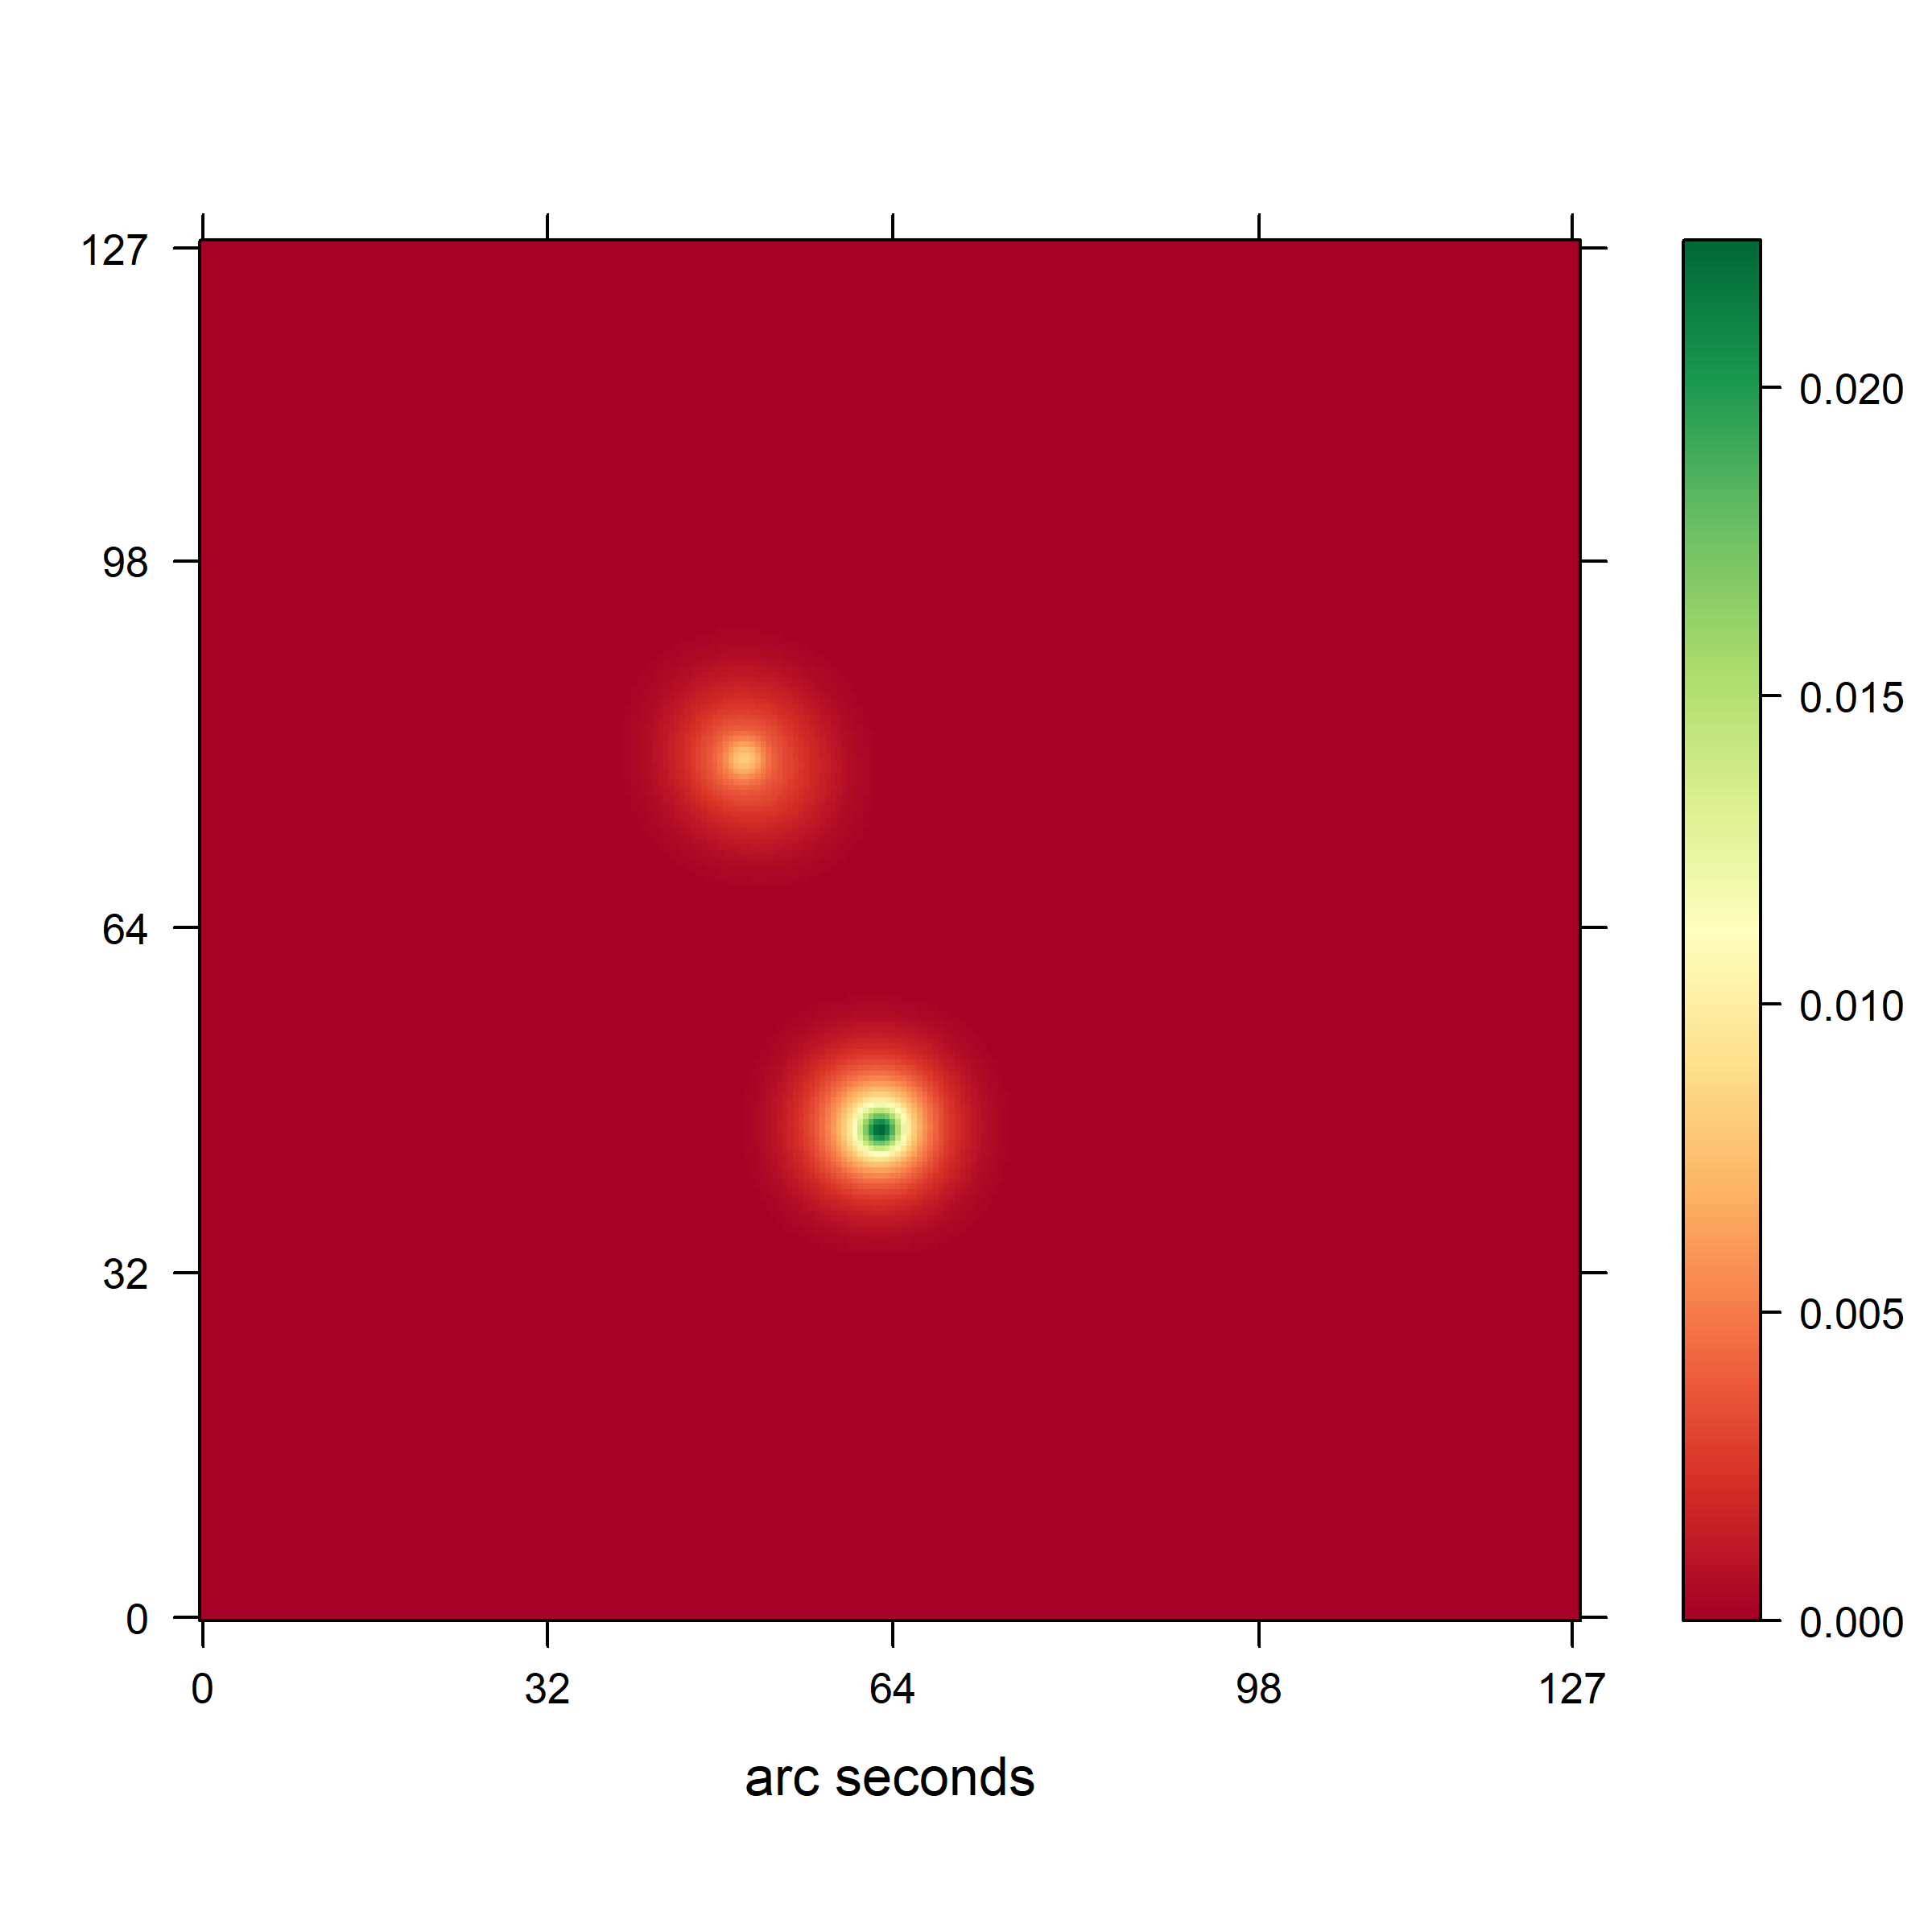
\includegraphics[width=\linewidth, trim={0.2in, 0.2in, 0, 0.2in}, clip]{./chapters/20.results/points/tclean_points.png}
		\caption{CLEAN reconstruction \\with CASA standard parameters.}
		\label{results:points:tclean}
	\end{subfigure}
	\begin{subfigure}[b]{0.4\linewidth}
		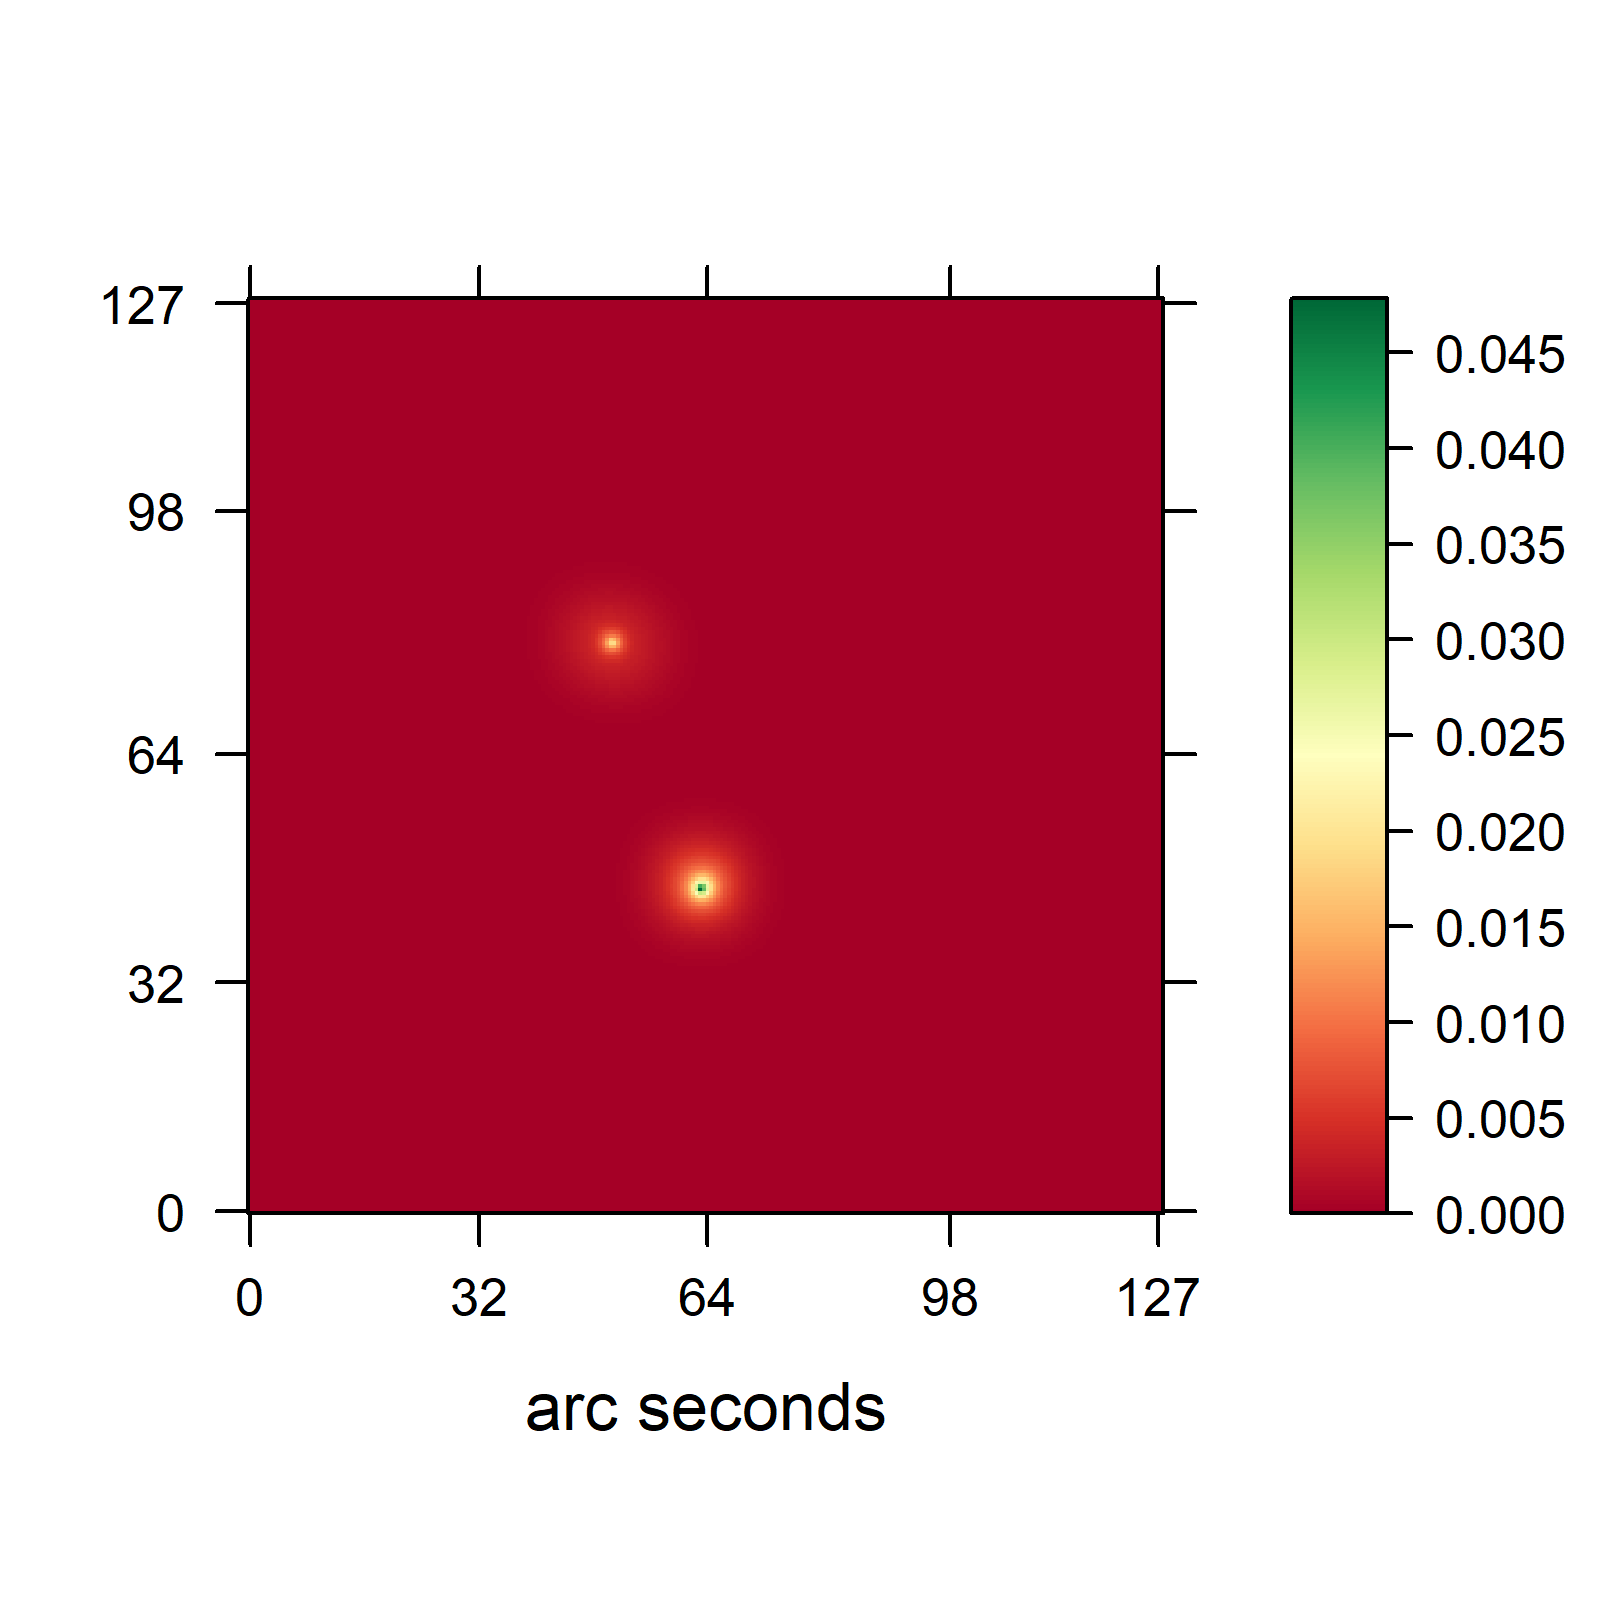
\includegraphics[width=\linewidth, trim={0.2in, 0.2in, 0, 0.2in}, clip]{./chapters/20.results/points/cd_points.png}
		\caption{Coordinate Descent reconstruction\\ with $\lambda = 0.1, J=3$.}
		\label{results:points:cd}
	\end{subfigure}
	
	\caption{Image reconstruction of two point sources.}
	\label{results:points}
\end{figure}

The total Flux of the image, the sum of all emissions, is 2.5+1.4 Jansky/Beam in this simulation. CLEAN reconstructs the right peak intensities, both ending up at 2.5 and 1.7 respectively. Since CLEAN reconstructs a blurred version, the total Flux of the image is off by magnitudes. Figure \ref{results:points:contour} compares the intensity profile of CLEAN, Coordinate Descent and the Ground Truth.

Intensity profile

\begin{figure}[h]
	\centering
	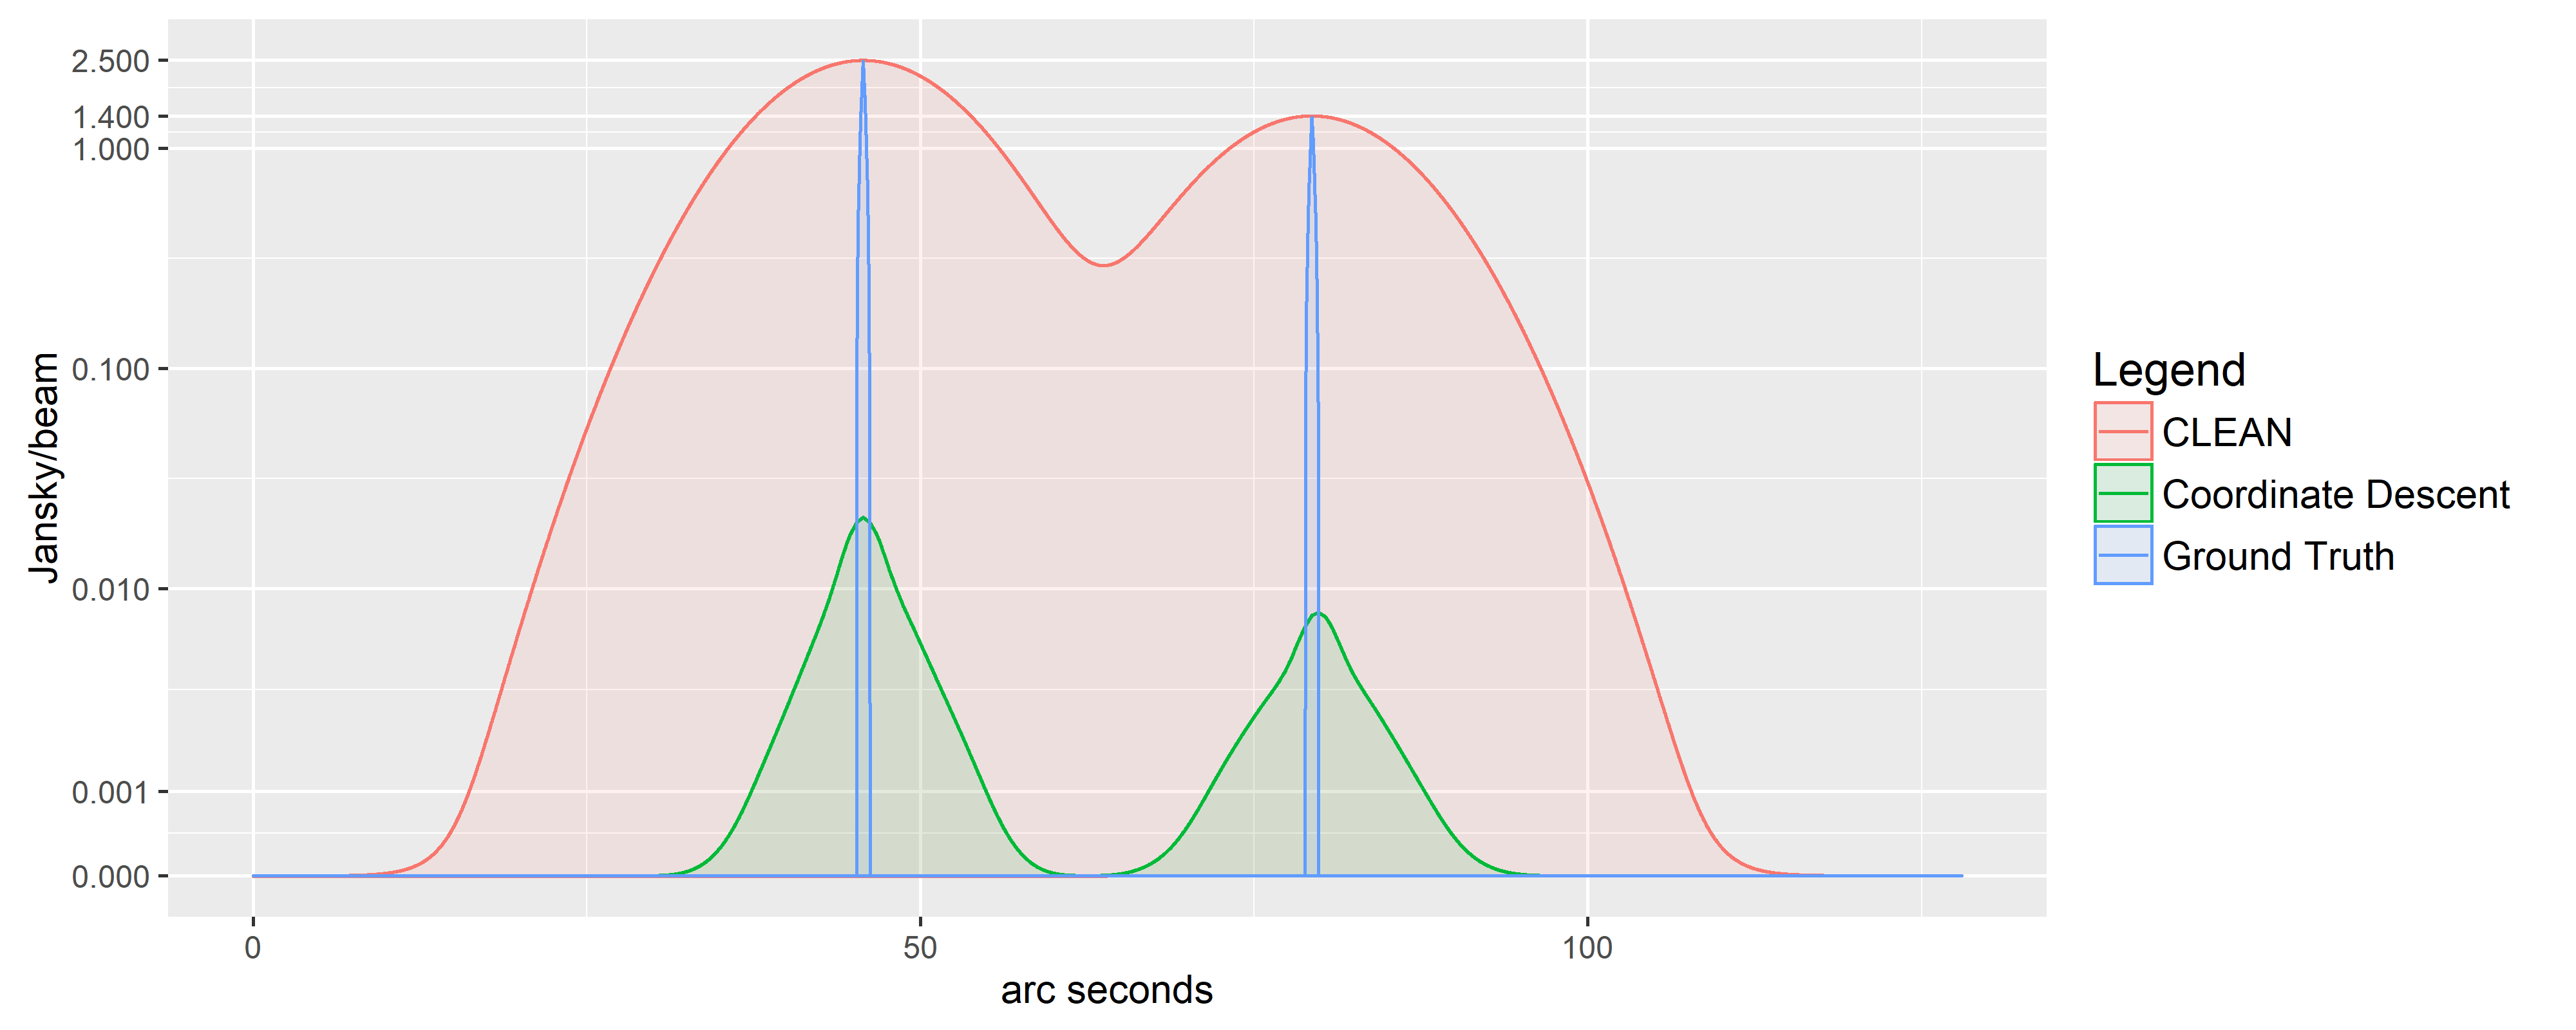
\includegraphics[width=0.8\linewidth]{./chapters/20.results/points/contour_points.png}
	\caption{Intensity profile of the two point sources.}
	\label{results:points:contour}
\end{figure}
		
Sparse representation, 192 non-zeros

intensity profile

Flux


issues with Coordinate descent reconstruction, wrong flux, lower peak is wider than, and is offest by approximately a pixel

Look at the flux in a more complex environment


\subsection{Flux reconstruction of mixed sources}


Parameters of Coordinate Descent

super resolution of CD. However, it did not find all point sources
Lets look closer at the flux reconstruction of extended emissions

\begin{figure}[h]
	\centering
	\begin{subfigure}[b]{0.4\linewidth}
		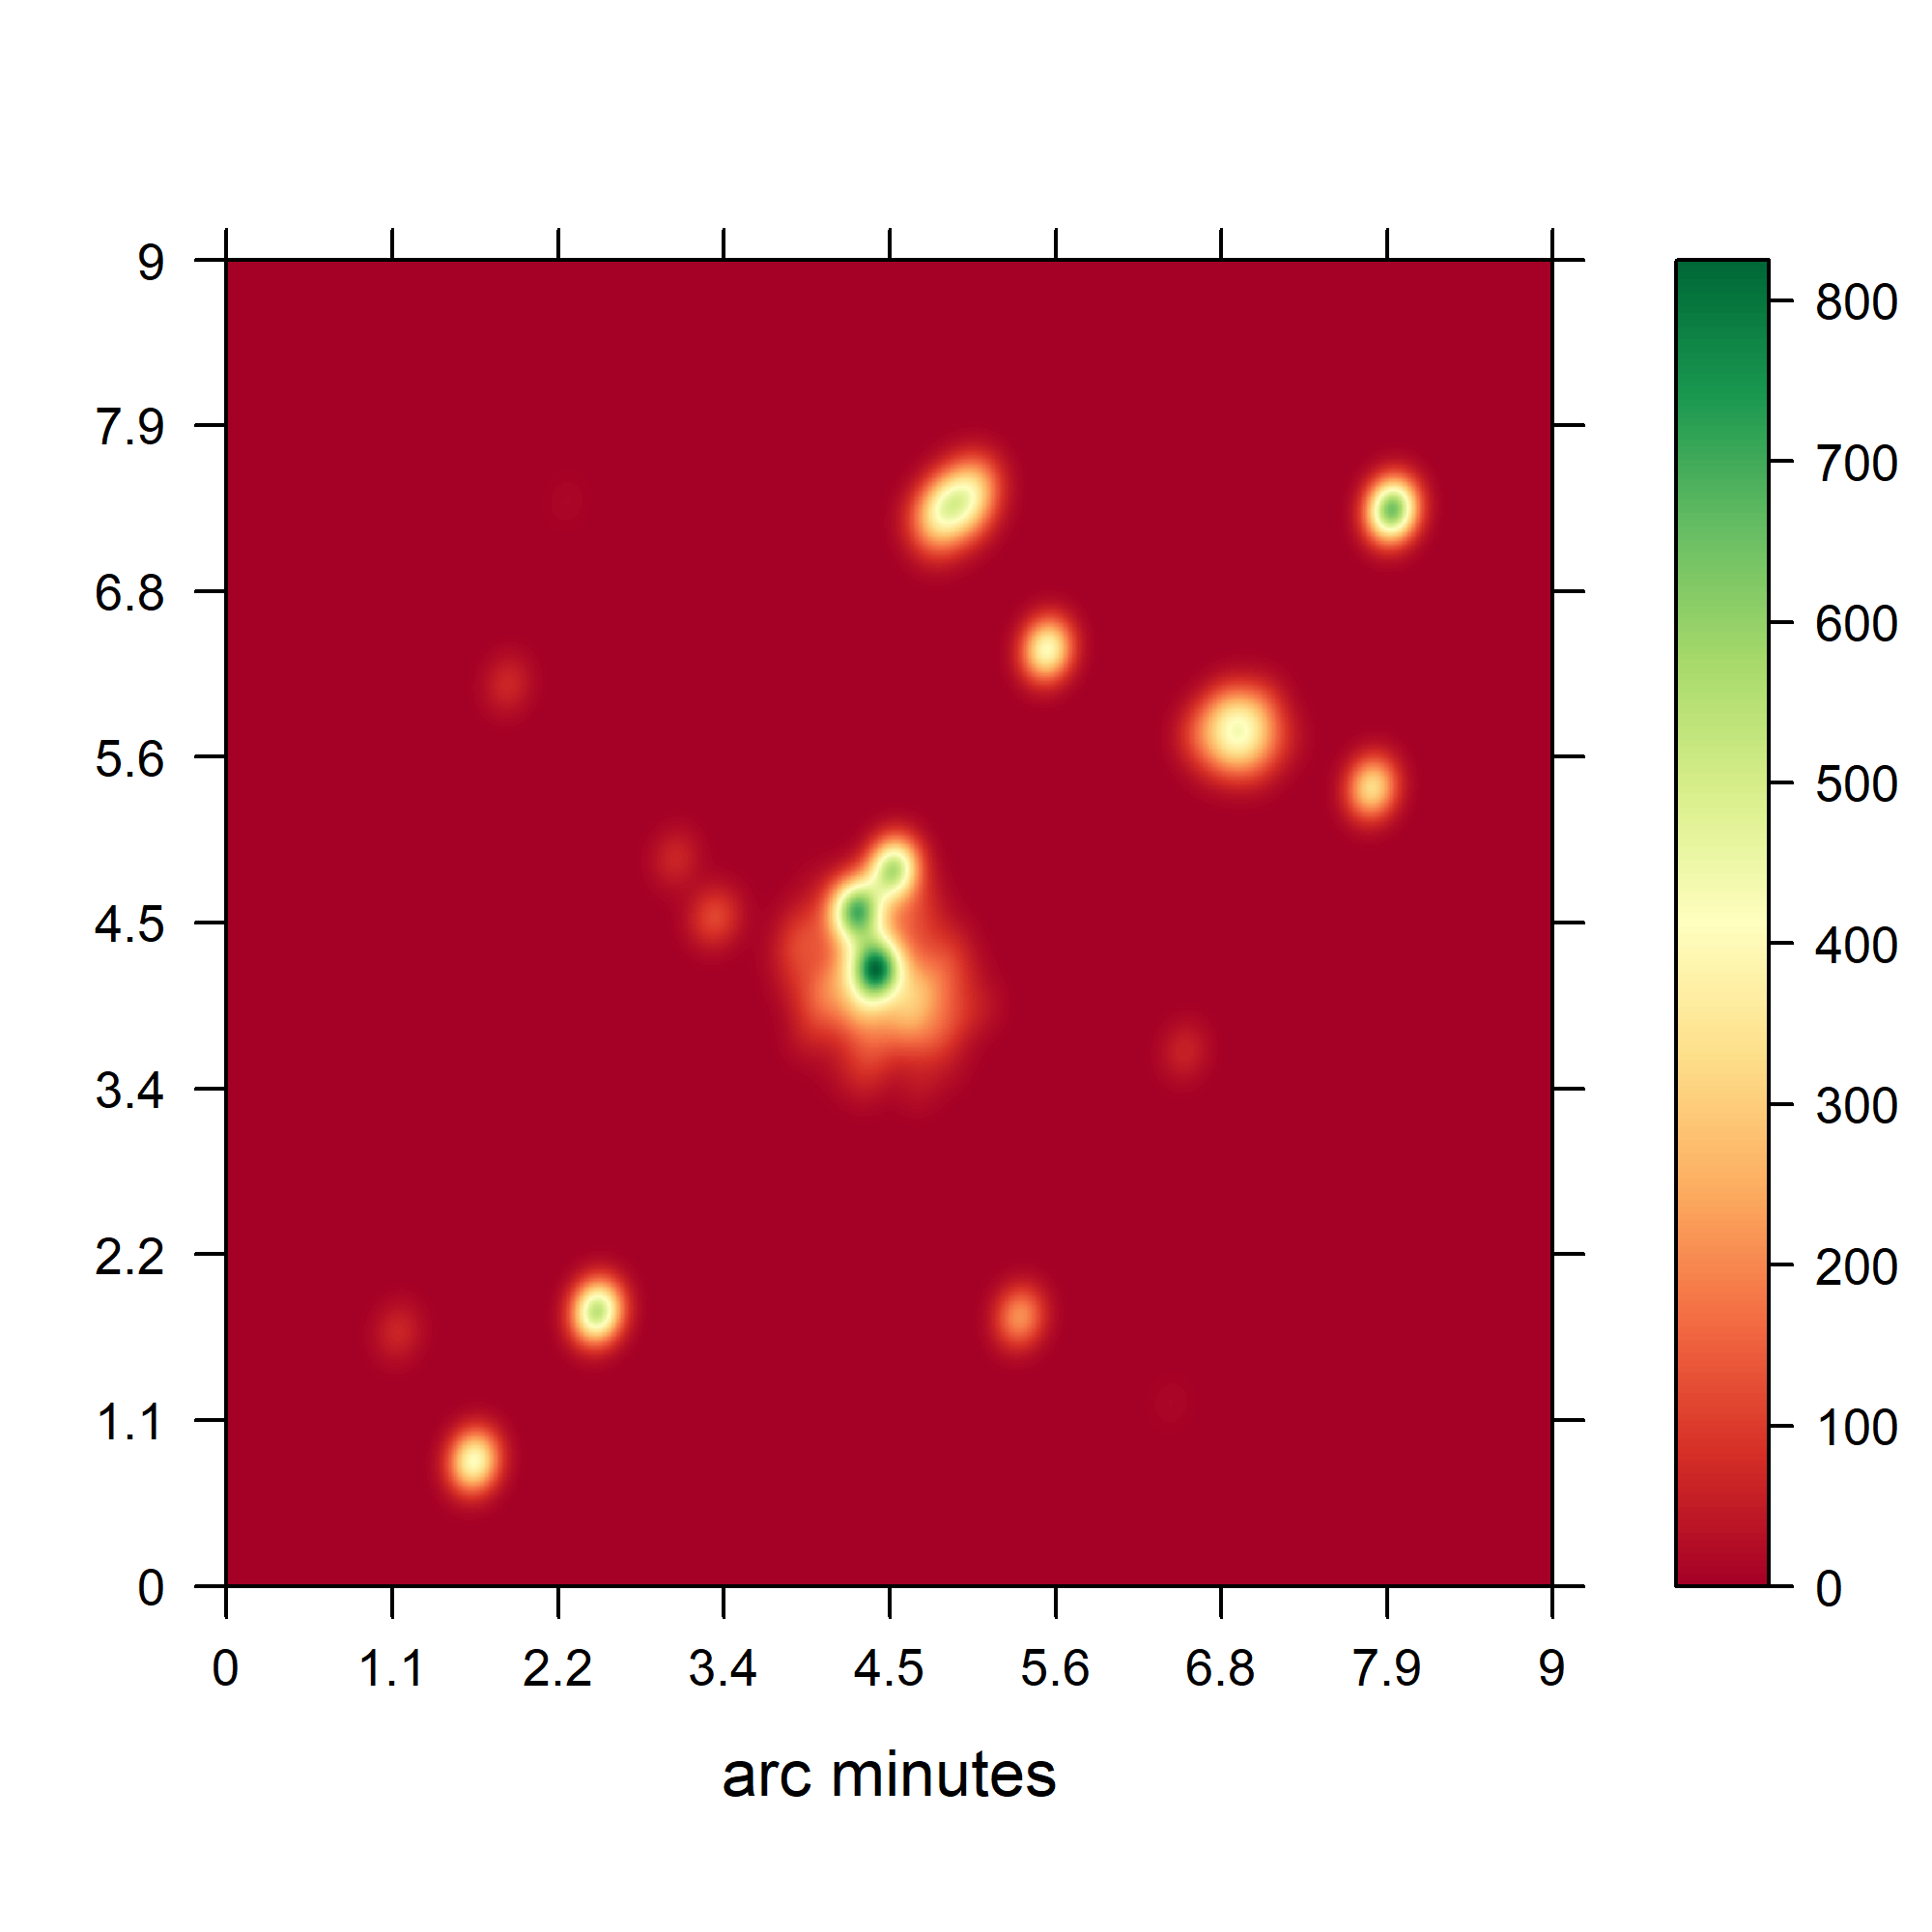
\includegraphics[width=\linewidth, trim={0.2in, 0.2in, 0, 0.2in}, clip]{./chapters/20.results/mixed/mixed_clean.png}
		\caption{CLEAN reconstruction}
		\label{results:mixed:tclean}
	\end{subfigure}
	\begin{subfigure}[b]{0.4\linewidth}
		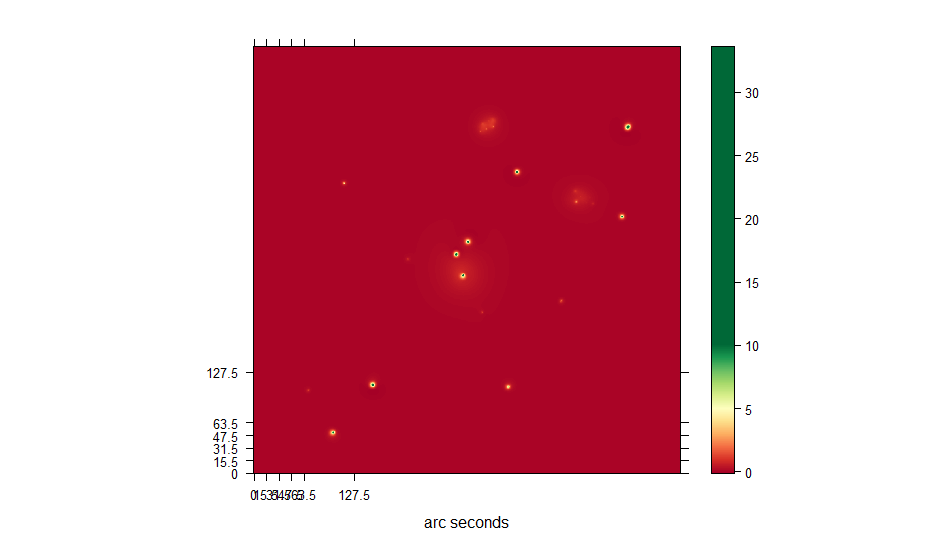
\includegraphics[width=\linewidth, trim={0.2in, 0.2in, 0, 0.2in}, clip]{./chapters/20.results/mixed/mixed_cd.png}
		\caption{Coordinate Descent Reconstruction}
		\label{results:mixed:cd}
	\end{subfigure}
	\caption{Reconstruction on mixed sources}
	\label{results:mixed}
\end{figure}

Question of Flux reconstruction

 $\lambda$ for different starlet layers like in \cite{girard2015sparse}

\begin{figure}[h]
	\centering
	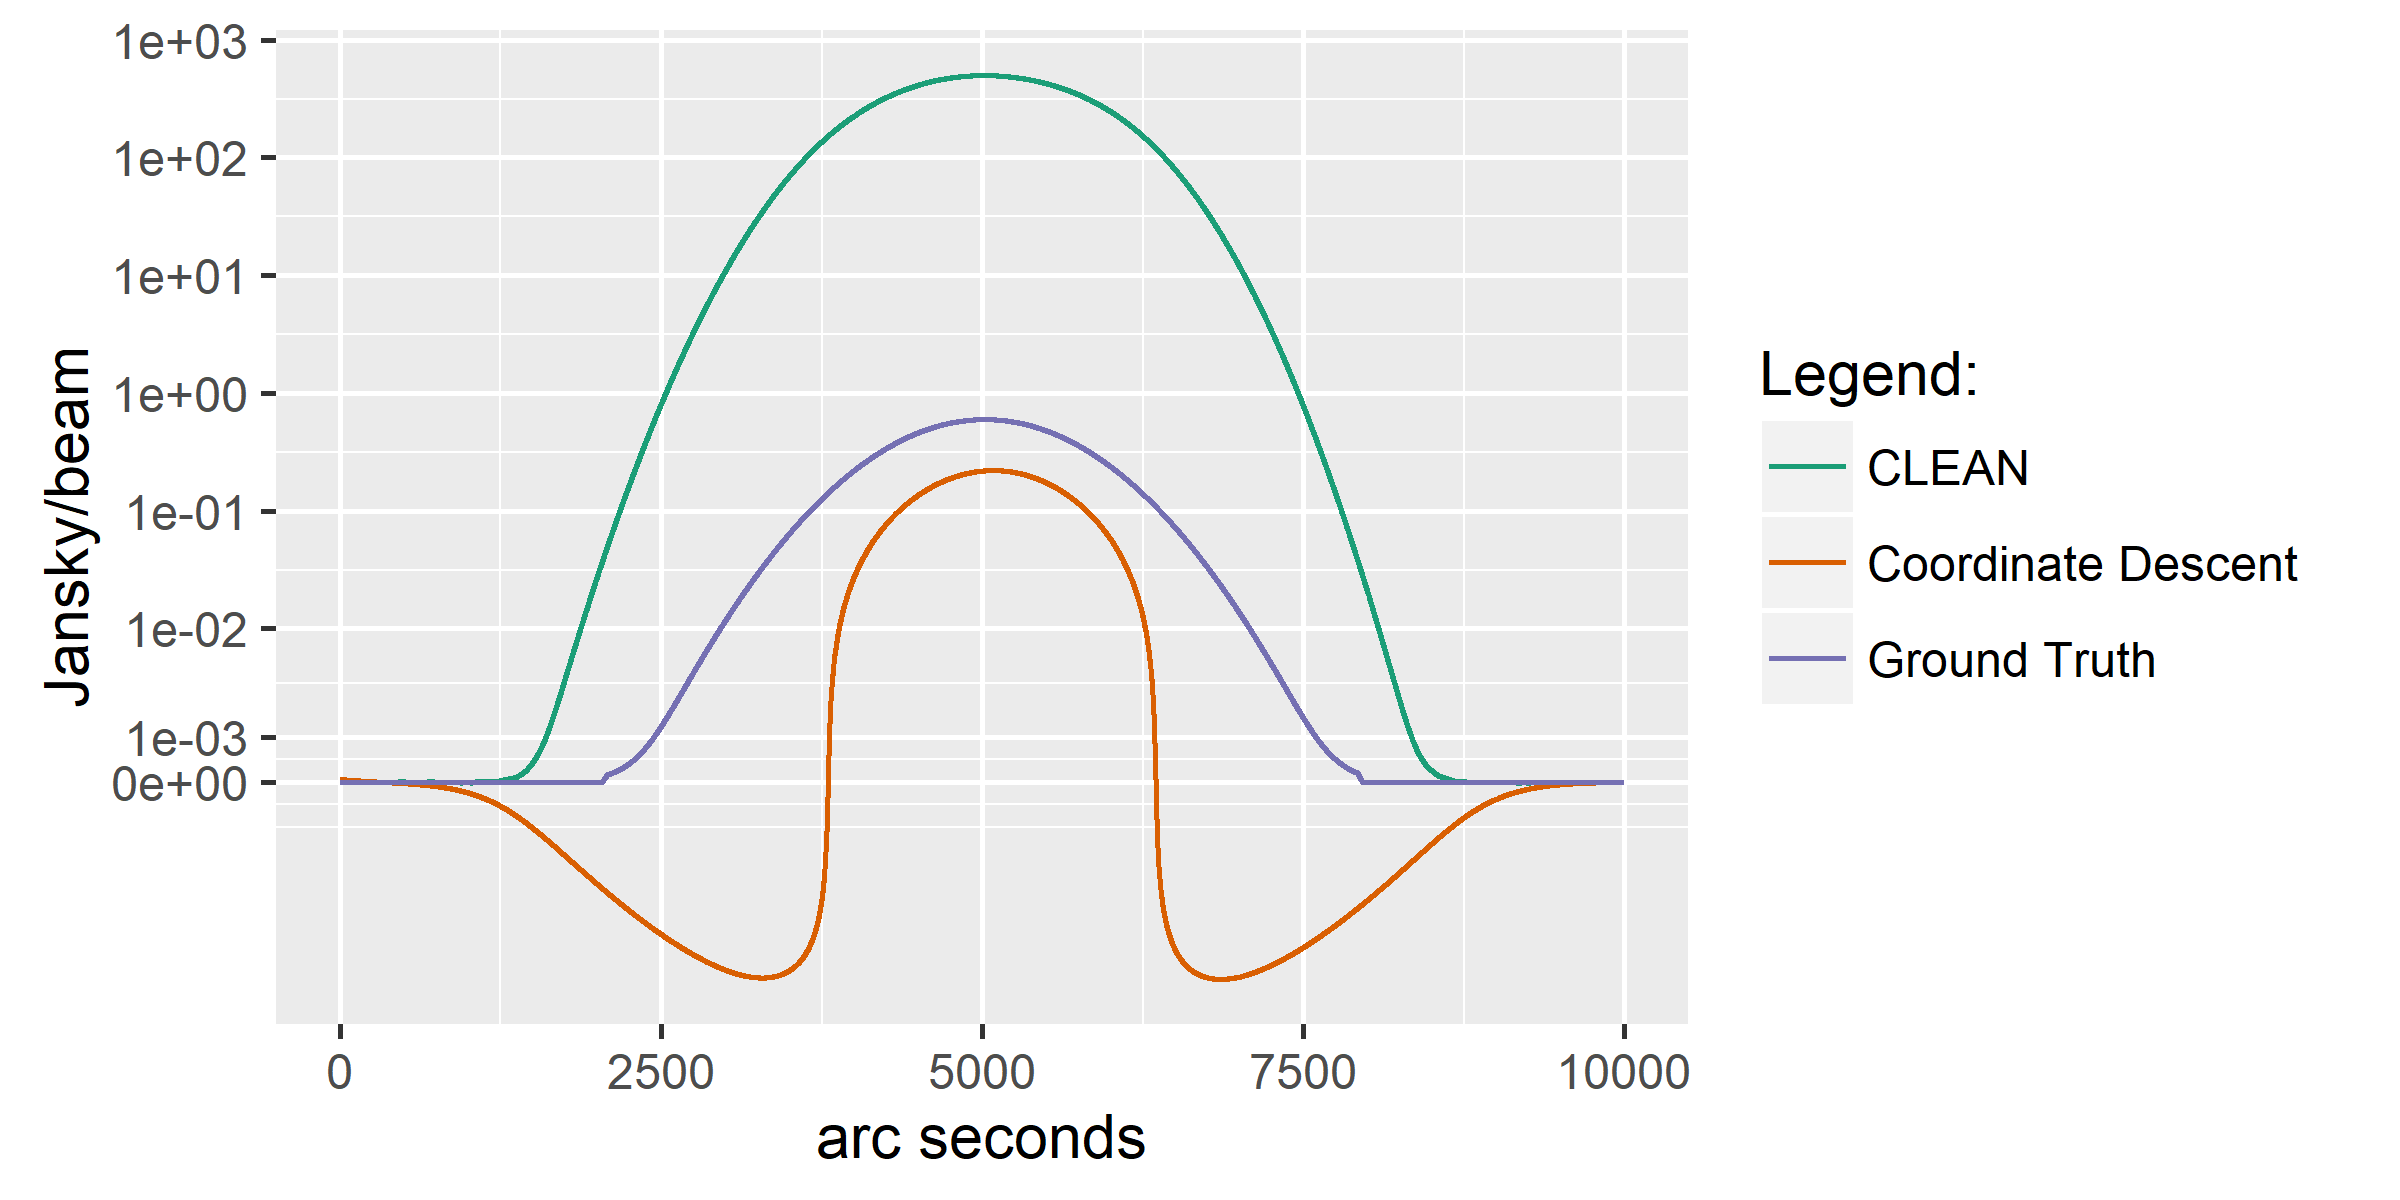
\includegraphics[width=0.8\linewidth]{./chapters/20.results/mixed/mixed_contour.png}
	\caption{Reconstruction on mixed sources}
	\label{results:mixed:contour}
\end{figure}

V

In this section, we compare the Coordinate Descent reconstruction with CLEAN on simulated MeerKAT data, and compare the runtime complexity of the two approaches on a real-world MeerKAT observation. We show that Coordinate Descent reconstructs the image by only computing a subset of the Fourier Transform Matrix' columns $F^{-1}$, and investigate if this approach reduces the runtime complexity on the large scale reconstruction problems of MeerKAT.


The real world MeerKAT data were calibrated and averaged down to reduce its size to 88 Gigabytes. The raw, uncalibrated data ranges between 500 and 1000 Gigabytes. Data on this scale requires a mature pipeline for reading and image reconstruction. Within the time limit of this project, only a reconstruction with the WSCLEAN\cite{offringa2014wsclean} pipeline was possible.

The simulations were created with the Meqtrees software package. Two simulations which contain roughly (size of Visibilities) perfectly calibrated Visibilities were created. 

\subsection{Imaging on Simulated Data}
We compare the reconstruction of Coordinate Descent and CLEAN on two simulated observations. The first observation contains two point sources, on which we show that Coordinate Descent is able to locate the sources below the accuracy limit of the instrument. The second observation contains point and Gaussian sources, on which we show that Coordinate Descent better captures the intensity profile of extended emissions. Also, we look at the shortcomings of the proof-of-concept implementations in terms of reconstruction quality and runtime. We use the CLEAN implementation of CASA in this section. CASA is an established software framework for radio interferometer image reconstruction and was already used in a previous project.


We used CASA's default parameters for CLEAN, except for the maximum number of CLEAN iterations, which we set to 250. The proof-of-concept Coordinate Descent implementation has three parameters to tune: Number of iterations, the number of starlet layers $J$, and the regularization parameter $\lambda$. The first two parameter could be estimated by the reconstruction algorithm itself. In this implementation, it was left to the user. For the two simulations the Coordinate Descent parameters were chosen:
\begin{itemize}
	\item Two Point sources: 4 full iterations, $J=3$, $\lambda=0.1$
	\item Mixed sources: 4 full iterations, $J=7$, $\lambda=0.1$
\end{itemize}

In figure \ref{results:point} shows an image of the Coordinate Descent and CLEAN reconstruction. Figure \ref{results:points:contour} shows the intensity profile of both reconstructions compared with the ground truth. Note that figure \ref{results:points:contour} has a logarithmic y axis. The reconstructions differ in two notable ways: The peak intensity of the source, and how much each algorithm spreads the point source. 

\textit{Spread}: CLEAN reconstructs a convolved version of the true image. CLEAN locates the two peaks in figure \ref{results:points:contour}, but convolves the point source with a Gaussian function. CLEAN reconstructs two Gaussian functions with same peak as the point source. The Gaussian represents the accuracy of the instrument. With compressed sensing, we try to reconstruct the observed image above the accuracy of the instrument. In the intensity profile, Coordinate Descent reconstructs two narrow gaussian-like peaks, essentially super-resolving the image. However, note that the total intensity is a fraction of the original peaks.

\textit{Intensity:} [Total Flux] The reconstructions differ in intensity. The figure \ref{results:points:contour} shows the intensity pr. Also note that Coordinate Descent has shifted the smaller peak by a pixel in its reconstruction. [Total flux correct in CD?]



The difference in intensity becomes more apparent with extended emissions. Figure \ref{results:mixed} shows Coordinate Descent and tCLEAN on the simulation with mixed sources. Again the two reconstructions arrive at different intensities. The gaussian emissions are reconstructed with a higher intensity than Coordinate Descent.






With starlets, coordinate descent has a representation for extended emissions. Looking at the intensity profile of an extended emisions \ref{}, we see Coordiante Descent coming closer to the true intensity. Although in the four iterations,  [it still had a considerable margin on error]. 



Coordinate Descent did not reconstruct all point sources. How many starlets are non-zero is the major point for runtime. It depends on how many areas of the image are non-zero. Starlet has a representation for extended emission, how many starlets are needed for modelling is hard.

Runtime problems
1900 non-zero starlets, 